\subsection{Aufbau und Wirkungsweise}
Ein Geiger-Müller-Zährohr besteht aus einem Kathodenzylinder mit Radius $r_{k}$. In diesem verläuft axial ein Anodendraht mit Radius $r_{a}$. Der Innenraum ist mit einem Gasgemisch gefüllt (Beispiel: 100 mbar Argon und 10 mbar Ethanol). Wird eine Spannung zwischen Kathode und Anode angelegt, ensteht ein radialsymmetrisches Feld mit dem Wert :\\
\begin{align}
E(r)=\frac{U}{r \ln(r_{k}/r_{a})}
\label{1}
\end{align}\\
	\begin{figure}[h]
		\begin{center}
		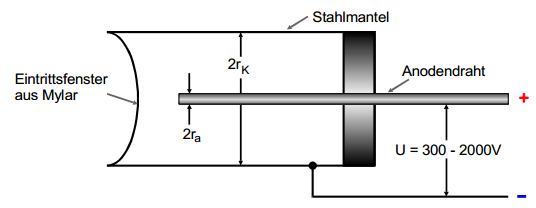
\includegraphics[scale=1.0]{Querschnitt.png}
		\caption{Querschnitt durch ein Endfenster-Zählrohr [1]}
		\label{Quer}
		\end{center}	
	\end{figure}\\
Eine Kopfseite des Zylinders besteht aus einer dünnen Schicht Material wie Mylar, durch welches die Teilchen eintreten können.\\
Tritt nun ein Teilchen in den Zylinder ein, wandert es durch den Raum und ionisiert die Gasmoleküle, bis seine Energie aufgebraucht ist. Die Anzahl der Ionisationen ist dabei proportional zur Energie des Teilchens. Die anschließenden Vorgänge hängen von der angelegten Spannung ab.
	\begin{figure}[h]
		\begin{center}
		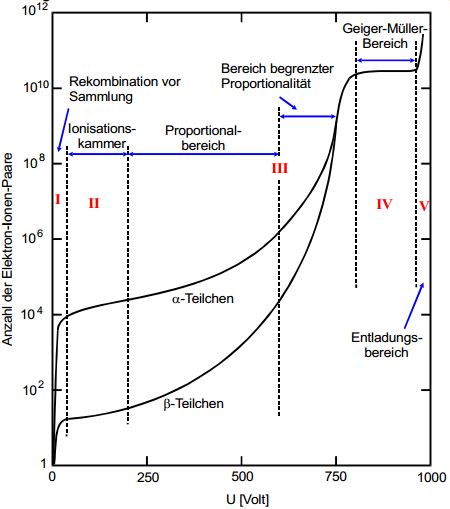
\includegraphics[scale=0.8]{Anzahl.png}
		\caption{Anzahl der Elektron-Ion-Paare in Abhängigkeit der angelegten Spannung U [1]}
		\label{Anzahl}
		\end{center}	
	\end{figure} \\
Bei sehr niedrigen Spannungen gelangen kaum Elektronen zum Draht, da diese sich meist vorher rekombinieren (Bereich I in Abb. \eqref{Anzahl}).
Im nächsten Abschnitt erreichen quasi alle Elektronen den Draht. Hier ist der Ionisationsstrom proportional zur Energie und Intensität der einfallenden Teilchen. Ein solcher Detektor wird Ionisationskammer genannt. Hier kann nur bei hohen Strahlungsintensitäten gemessen werden (Bereich II in Abb. \eqref{Anzahl}).\\
Bei weiterer Spannungserhöhung können die ausgelösten Elektronen ihrerseits ionisieren. Dies wird Stoßionisation genannt. Dies erzeugt eine Townsend-Lawine, da auch die so erzeugten Elektronen ionisieren können. Die Proportionalität zur Energie bleibt erhalten.
Man bezeichent das Zählrohr in diesem Bereich als Proportionalitätszählrohr (Bereich III in Abb. \eqref{Anzahl}).\\
An diesen Bereich schließt sich der Auslösebereich an. Hier arbeitet der Geiger-Müller-Zähler. Durch entstehende UV-Photonen bei Anregung der Argon-Teilchen, welche sich aufgrund ihrer Ladungsneutralität im ganzen Zählrohr ausbreiten können, entstehen Elektronenlawinen im ganzen Zählrohr. Die am Draht gesammelte Ladung hängt nur noch von der Geometrie des Zählrohres ab. So lässt sich nur noch die Intensität messen (Bereich IV in Abb. \eqref{Anzahl}). 

\subsection{Vorteile und Nachteile des Geiger-Müller-Zählrohrs}
Der größte Vorteil ist seine breite Einsatzmöglichkeit aufgrund seiner einfachen Handhabbarkeit, da man nur wenige weitere elektrische Geräten benötigt und es sehr kompakt ist.Es kann so auch im Freien eingesetzt werden.
Auch sein hohes Ansprechvermögen für $\alpha$- und $\beta$-Strahlung, zudem im selben Arbeitsbereich, zeichnet es gegenüber anderen Detektoren aus.
Der 1. Nachteil des Geiger-Müller-Zählrohrs ist die Totzeit. Diese hat zur Folge, dass während dieser Zeit eintretende Teilchen nicht registriert werden können.
Die Totzeit entsteht, da die positiven Ionen wesentlich langsamer zum Draht wandern aufgrund ihrer deutlich höheren Masse. Diese erzeugen eine radialsymmetrische, positive Raumladung. Die Feldstärke in Drahtnähe fällt dadurch so stark ab, dass keine Stoßionisation möglich ist. An die Totzeit schließt sich die Erholungszeit an, in welcher zwar Ladungsimpulse registriert werden,allerdings nicht in der vorherigen Größe. Diese wird erst wieder erreicht, wenn die Ionen neutralisiert sind. Den Verlauf von Tot- und Erholungszeit sieht man in Abb. \eqref{Tot} 
	\begin{figure}[h]
		\begin{center}
		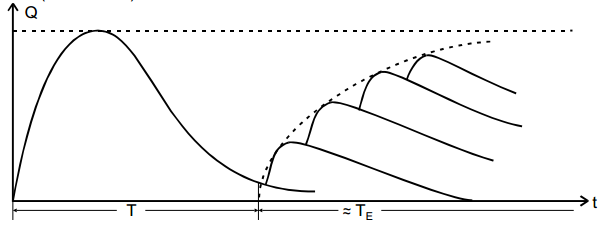
\includegraphics[scale=0.8]{Totzeit.png}
		\caption{Verlauf von Tot- und Erholungszeit [1]}
		\label{Tot}
		\end{center}	
	\end{figure} \\
Ein weiterer Nachteil ist der Effekt der Nachentladungen. Diese entstehen durch Sekundärelektronen, welche beim Auftreffen der Ionen auf die Zählrohrwand von diesen aus der Metalloberfläche gelöst werden. Da dieser Vorgang länger dauert als die Totzeit, werden die Sekundärelektronen als weiterer Impuls gezählt. Dies ist höchst unerwünscht. Der Effekt lässt sich minimieren durch den Zusatz von Alkoholdämpfen ins Zählrohr. Die Edelgasionen ionisieren die Alkoholmoleküle auf ihrem Weg zur Kathodenwand. Die Alkoholionen wandern nun zur Wand, an welcher sie neutralisiert werden. Dabei wird allerdings kein weiteres Elektron ausgelöst, da die Energie zur Anregung von Schwingungen des Moleküls verbraucht wird.
\subsection{Charakteristik des Zählrohrs}
Als Charakteristik des Zählrohres bezeichnet man die Kurve die entsteht, wenn bei konstanter Strahlungsintensität die Zahl der registrierten Teilchen $N$ gegen die ans Zählrohr angelegte Spannung $U$ aufgetragen wird. 
	\begin{figure}[h]
		\begin{center}
		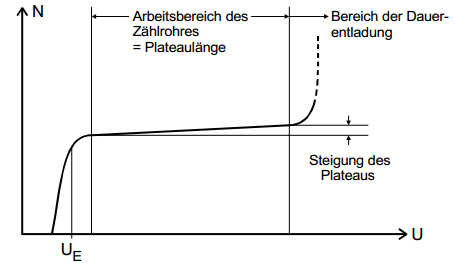
\includegraphics[scale=0.8]{Zahlrohrcharakteristik.png}
		\caption{Zählrohrcharakteristik [1]}
		\label{Zähl}
		\end{center}	
	\end{figure}
Wie in Abb. \eqref{Zähl} zu sehen ist setzt bei $U_{E}$ der Auslösebereich ein. Der daran anschließende lineare Bereich wird Plateau gennant. In diesem ist  $N$ nahezu konstant. Der Plateauanstieg sollte bei einem guten Zählrohr möglichst klein sein über einen möglichst breiten Bereich. Der Anstieg entsteht durch vereinzelte Nachentladungen. 
\subsection{Ansprechvermögen des Zählrohrs}
Als Ansprechvermögen eines Zählrohrs wird die Empfindlichkeit für bestimmte Teilchen und Quanten bezeichnet. So  ist das Ansprechvermögen des Geiger-Müller-Zählrohrs für $\alpha$- und $\beta$-Strahlung nahezu 100 \% aufgrund ihres hohen Ionisationsvermögens. Da Photonen nur sehr gering wechselwirken, beträgt ihr Ansprechvermögen nur etwa 1\%. Daher eignet sich ein Geiger-Müller-Zählrohr nur für hohe Intensitäten an $\gamma$-Strahlung.
